%!TEX program = xelatex
\documentclass{article}
\usepackage[a4paper,left=2.5cm,right=2.5cm,top=2.2cm,bottom=2.2cm]{geometry}
\usepackage{listings}
\usepackage{float}
\usepackage{graphicx}
\usepackage{xcolor}
\usepackage{amsmath}
\usepackage{amssymb}
\usepackage{siunitx}
\usepackage{booktabs}
\usepackage[most]{tcolorbox}
\usepackage{tikz}
\usepackage{pgfplots}
\usepgfplotslibrary{groupplots}

\pgfplotsset{compat=1.18}

\sisetup{per-mode=reciprocal, inter-unit-product = \cdot}

% Solution formatting (distinct from prompts)
\newtcolorbox{solutionbox}{
    enhanced,
    breakable,
    boxrule=0.6pt,
    colframe=blue!35,
    colback=blue!6,
    arc=2mm,
    left=1.2mm,
    right=1.2mm,
    top=1.0mm,
    bottom=1.0mm,
}
% By default, each solution starts on a new page. For special cases (e.g., keep a prompt
% and its solution on the same page), call \nosolutionpagebreak right before \begin{solution}.
\newif\ifsolutionclearpage
\solutionclearpagetrue
\newcommand{\nosolutionpagebreak}{\global\solutionclearpagefalse}
\newenvironment{solution}{%
    \ifsolutionclearpage\clearpage\fi
    \global\solutionclearpagetrue
    \par\noindent\begin{solutionbox}\textbf{\textit{Solution.}}\par\medskip\itshape
}{%
    \end{solutionbox}
}

% Disable equation numbering globally (match the unnumbered style used earlier)
\let\numberedequation\equation
\let\endnumberedequation\endequation
\renewenvironment{equation}{\begin{equation*}}{\end{equation*}}

\title{\textbf{Spring'\ 26 \; Introduction to Biological Intelligence: Brain Simulation\\ \textcolor{red}{Project 1 Part 1} Derivation \& Calculation}}
\author{}
\date{}

\begin{document}
\pagestyle{plain}
\maketitle

\vspace{-3.5em}

\begin{center}
\Large
\textbf{Yian Li (PKU, 2300017854)}\\
\textbf{ZiHang Xu (THU, 2023010082)}\\
\textbf{WeiJun Hong (PKU, 2400017452)}
\end{center}
\vspace{0.5em}

\section{Response of an RC Neuron to Injected Current}

As we derived in class, when a constant current $I_0$ (an ideal current source) is injected into a passive neuron (modeled as an RC circuit) at $t=0$, starting from the resting state,
the membrane potential $V_m(t)$ will exponentially decay towards the steady state
\[
V_{\infty}=V_{\text{rest}} + RI_0,
\] as illustrated below:

\begin{figure}[H]
    \centering
    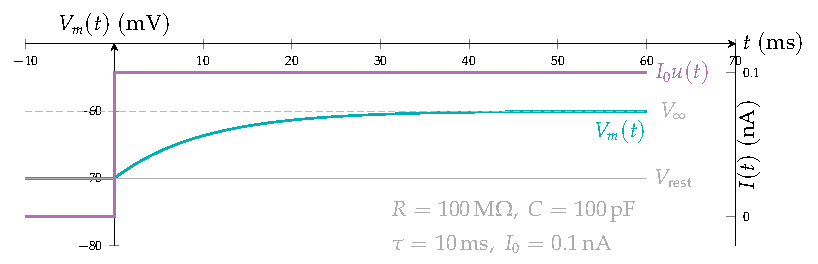
\includegraphics[width=0.8\linewidth]{Unit_step_resp.pdf}
\end{figure}

Now suppose that at some later time $t_0$ the input current $I_0$ is removed. 
Derive how the membrane potential evolves after this moment.
Note that at time $t_0$ the membrane potential $V_m$ has not yet reached the steady-state value $V_{\text{rest}} + RI_0$, and this should not be ignored in your derivation.
(\textit{Hint:}  You may either solve the corresponding ODE directly, or compute the response using the impulse response of the RC circuit convolved with the injected current.)\\

Now consider a periodic input with period $T$, where during the first $t_0 \ll T$ portion of each cycle a current $I_0$ is injected.
Describe how the membrane potential evolves in this situation, and from this perspective explain why an RC neuron behaves as a \textbf{low-pass filter}.
(\textit{Hint:} When considering the range of $t_0$, you may take the membrane time constant $\tau$ as a reference scale. You may assume that by the end of each period $T$ the neuron has returned to its resting potential.)

\begin{solution}
\textbf{1. Evolution of the membrane potential after $t_0$.}
During the current injection ($0\le t\le t_0$), the membrane potential charges towards the steady state $V_{\text{rest}}+RI_0$.
At the moment $t_0$ when the current is removed, the membrane potential is
\[
V_m(t_0)=V_{\text{rest}}+RI_0\left(1-\mathrm{e}^{-\frac{t_0}{\tau}}\right).
\]
For $t>t_0$, the injected current becomes zero and the passive membrane discharges through the leak resistance. The governing ODE is
\[
\tau\frac{\mathrm{d}V_m}{\mathrm{d}t}=-(V_m-V_{\text{rest}}).
\]
Solving with the initial condition $V_m(t_0)$ gives an exponential return to rest:
\[
V_m(t)=V_{\text{rest}}+\bigl[V_m(t_0)-V_{\text{rest}}\bigr]\,\mathrm{e}^{-\frac{t-t_0}{\tau}},\qquad t>t_0.
\]

\textbf{2. Periodic input and the low-pass filter property.}
For a periodic current pulse of duration $t_0\ll T$, if $t_0\ll\tau$ then the capacitor cannot charge much within a single pulse.
Therefore $V_m$ increases only slightly during the brief injection and then decays back toward $V_{\text{rest}}$ during the remainder of the period.

This illustrates the \textbf{low-pass} behavior: the membrane time constant $\tau$ sets how fast the voltage can track changes in input.
Fast (high-frequency) fluctuations are attenuated because the membrane does not have time to charge/discharge fully, whereas slow (low-frequency) inputs allow $V_m$ to follow the input more closely.

\medskip
\textbf{Illustration (computed from the piecewise ODE solution for periodic pulses).}
Assume a periodic pulse train with period $T$, and within each period the current is injected only for the first
$t_0=\alpha T$ with $\alpha\ll 1$ (e.g., $\alpha=0.1$). Within each period, the analytic piecewise solution takes the form
\[
\frac{V_m(t)-V_{\text{rest}}}{RI_0}=
\begin{cases}
1-\mathrm{e}^{-\frac{t}{\tau}}, & 0\le t\le t_0,\\
\bigl(1-\mathrm{e}^{-\frac{t_0}{\tau}}\bigr)\,\mathrm{e}^{-\frac{t-t_0}{\tau}}, & t_0<t\le T.
\end{cases}
\]
Because $t_0$ scales with $T$, a larger $T$ (lower frequency) gives a longer charging time and thus a larger peak depolarization.
To plot a clean periodic waveform (rather than assuming complete return to rest), we evaluate the \emph{periodic steady state} implied by this same analytic charging/discharging solution.

\begin{figure}[H]
\centering
\begin{tikzpicture}
\begin{axis}[
        width=0.92\linewidth,
    height=0.28\textheight,
        xmin=0, xmax=36,
    ymin=0, ymax=1.05,
    grid=both,
        xlabel={$t/\tau$},
    ylabel={$\bigl(V_m-V_{\text{rest}}\bigr)/(RI_0)$},
    legend style={draw=none, fill=none, font=\small},
    legend pos=north west,
]
\def\alpha{0.1}

% r = T/tau. Use periodic steady state for v0 at the start of each cycle.
% Let a = exp(-alpha*r), b = exp(-(1-alpha)*r).
% Then v0 = (1-a)*b/(1-a*b).
% Within each cycle (u = mod(t/tau, r)):
%   if u <= alpha*r: v = 1 + (v0-1)*exp(-u)
%   else:           v = v1*exp(-(u-alpha*r)) where v1 = 1 + (v0-1)*a

\pgfmathsetmacro{\r}{3}
\pgfmathsetmacro{\a}{exp(-\alpha*\r)}
\pgfmathsetmacro{\b}{exp(-(1-\alpha)*\r)}
\pgfmathsetmacro{\vzero}{(1-\a)*\b/(1-\a*\b)}
\pgfmathsetmacro{\vone}{1+(\vzero-1)*\a}
\addplot[thick, blue!75!black, samples=1600, domain=0:36]
    {(mod(x,\r)<=\alpha*\r) ? (1+(\vzero-1)*exp(-mod(x,\r))) : (\vone*exp(-(mod(x,\r)-\alpha*\r)))};
\addlegendentry{$T/\tau=3$ (higher freq)}

\pgfmathsetmacro{\r}{6}
\pgfmathsetmacro{\a}{exp(-\alpha*\r)}
\pgfmathsetmacro{\b}{exp(-(1-\alpha)*\r)}
\pgfmathsetmacro{\vzero}{(1-\a)*\b/(1-\a*\b)}
\pgfmathsetmacro{\vone}{1+(\vzero-1)*\a}
\addplot[thick, teal!70!black, samples=1600, domain=0:36]
    {(mod(x,\r)<=\alpha*\r) ? (1+(\vzero-1)*exp(-mod(x,\r))) : (\vone*exp(-(mod(x,\r)-\alpha*\r)))};
\addlegendentry{$T/\tau=6$}

\pgfmathsetmacro{\r}{12}
\pgfmathsetmacro{\a}{exp(-\alpha*\r)}
\pgfmathsetmacro{\b}{exp(-(1-\alpha)*\r)}
\pgfmathsetmacro{\vzero}{(1-\a)*\b/(1-\a*\b)}
\pgfmathsetmacro{\vone}{1+(\vzero-1)*\a}
\addplot[thick, orange!85!black, samples=1600, domain=0:36]
    {(mod(x,\r)<=\alpha*\r) ? (1+(\vzero-1)*exp(-mod(x,\r))) : (\vone*exp(-(mod(x,\r)-\alpha*\r)))};
\addlegendentry{$T/\tau=12$ (lower freq)}

\end{axis}
\end{tikzpicture}
\caption{Voltage waveform $V_m(t)$ under periodic pulse injection, computed from the analytic piecewise solution in periodic steady state (fixed duty ratio $\alpha=t_0/T=0.1$). Larger $T$ (lower frequency) yields a larger peak depolarization.}
\end{figure}
\end{solution}







\clearpage

\section{Shunting Inhibition at Synapses}

Consider adding both an excitatory synaptic input (with reversal potential $E_e$) and a shunting inhibitory synaptic input (with reversal potential $E_i \approx V_{\text{rest}}$) to the RC circuit.
Assume that the postsynaptic conductances $g_e$ and $g_i$ are constant in time.
Write down the membrane equation after including these synaptic inputs. Derive expressions for:

\begin{itemize}
\item the new the input conductance $G_{\text{in}}$,
\item the new the time constant in the presence of synaptic input $\tau$,
\item the steady-state membrane potential $V_{\infty}$.
\end{itemize}

Now consider increasing $g_i$ from zero. How do the above quantities change?
Use your results to explain the mechanism of \textbf{shunting inhibition}.

\begin{figure}[H]
    \centering
    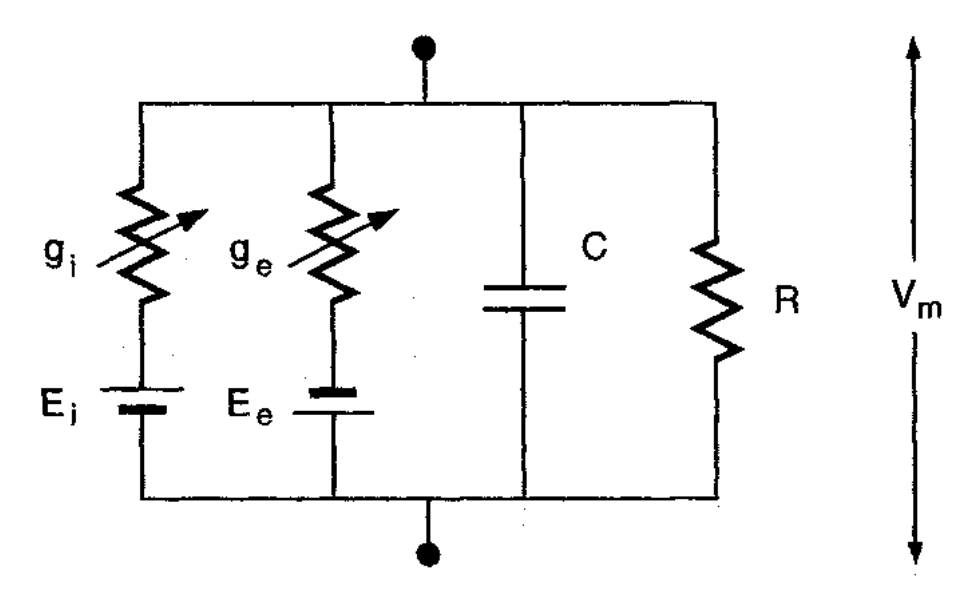
\includegraphics[width=0.6\linewidth]{RC_shunting.png}
\end{figure}

\begin{solution}
\textbf{1. Membrane equation.}
By Kirchhoff's current law, the capacitive current plus the leak current plus the synaptic currents sum to zero (including the resting potential offset for the leak):
\[
C\frac{\mathrm{d}V_m}{\mathrm{d}t}=-\frac{V_m-V_{\text{rest}}}{R}-g_e\,(V_m-E_e)-g_i\,(V_m-E_i).
\]

\textbf{2. Derivation of $G_{\text{in}}$, $\tau$, and $V_{\infty}$.}
Group the $V_m$ terms:
\[
C\frac{\mathrm{d}V_m}{\mathrm{d}t}=-\left(\frac{1}{R}+g_e+g_i\right)V_m+\left(\frac{V_{\text{rest}}}{R}+g_eE_e+g_iE_i\right).
\]
Hence the effective input conductance is
\[
G_{\text{in}}=\frac{1}{R}+g_e+g_i,
\]
and the effective membrane time constant becomes
\[
\tau=\frac{C}{G_{\text{in}}}=\frac{C}{\frac{1}{R}+g_e+g_i}.
\]
Setting $\frac{\mathrm{d}V_m}{\mathrm{d}t}=0$ gives the steady-state voltage
\[
V_{\infty}=\frac{\frac{V_{\text{rest}}}{R}+g_eE_e+g_iE_i}{\frac{1}{R}+g_e+g_i}.
\]

\textbf{3. Shunting inhibition mechanism.}
Increasing $g_i$ from zero gives the following monotonic changes:
\[
g_i\uparrow\quad\Longrightarrow\quad
G_{\text{in}}=\frac{1}{R}+g_e+g_i\uparrow
\quad\Longrightarrow\quad
\tau=\frac{C}{G_{\text{in}}}\downarrow.
\]
If $E_i\approx V_{\text{rest}}$, then the steady state simplifies to
\[
V_{\infty}\approx
\frac{\frac{V_{\text{rest}}}{R}+g_eE_e+g_iV_{\text{rest}}}{\frac{1}{R}+g_e+g_i}
=
V_{\text{rest}}+\frac{g_e\,(E_e-V_{\text{rest}})}{\frac{1}{R}+g_e+g_i}.
\]
Hence the depolarizing offset above rest satisfies
\[
\Delta V_{\infty}:=V_{\infty}-V_{\text{rest}}
\approx \frac{g_e\,(E_e-V_{\text{rest}})}{\frac{1}{R}+g_e+g_i}
\quad\Longrightarrow\quad
g_i\uparrow\;\Rightarrow\;\Delta V_{\infty}\downarrow.
\]
Equivalently, the same excitatory drive produces a smaller voltage change because the effective conductance is larger:
\[
\Delta V\sim \frac{I_e}{G_{\text{in}}},
\qquad
G_{\text{in}}\uparrow\;\Rightarrow\;\Delta V\downarrow.
\]
This is \textbf{shunting inhibition}: inhibition mainly increases conductance (a ``leak''/shunt) rather than strongly hyperpolarizing the cell.
\end{solution}

\clearpage

\section{The Nernst Equation}

In class we briefly derived the Nernst equation:

\[
E_k=\dfrac{RT}{zF}\ln\dfrac{[k]_o}{[k]_i}.
\]

Here

\begin{itemize}
    \item $R$ is the universal ideal gas constant: \SI{8.314}{\joule\per\kelvin\per\mole}
    \item $T$ is the temperature: \SI{300}{\kelvin}
    \item $F$ is the Faraday's constant: \SI{96485}{\coulomb\per\mol}
    \item $z$ is the ionic valence (for example, $z=+1$ for sodium)
\end{itemize}

Using the approximate intracellular and extracellular ion concentrations provided in the table below, compute the reversal potentials for the four major ions.

\begin{table}[H]
    \centering
    \begin{tabular}{lcc}
      \toprule
      & Extracellular (\si{\milli\mole\per\liter}) & Intracellular (\si{\milli\mole\per\liter}) \\
      \midrule
      $\mathrm{Na}^+$     & $\sim 140$ & $\sim 10$\\
      $\mathrm{K}^+$      & $\sim 4$   & $\sim 140$\\
      $\mathrm{Cl}^-$     & $\sim 120$ & $\sim 10$ \\
      $\mathrm{Ca}^{2+}$  & $\sim 1.5$ & $\sim 1.0\times10^{-4}$\\
      \bottomrule
    \end{tabular}
  \end{table}


Note that the Nernst equation describes the equilibrium potential for a \textbf{single ion species}. 
When the membrane is permeable to more than one ion, as is inevitably the case, how can the resting potential be determined?
Interested students may look up the \textbf{Goldman equation}. (No written answer is required.)

\begin{solution}
First compute the constant factor:
\[
\frac{RT}{F}=\frac{\SI{8.314}{\joule\per\kelvin\per\mole}\cdot\SI{300}{\kelvin}}{\SI{96485}{\coulomb\per\mole}}\approx \SI{0.02585}{\volt}=\SI{25.85}{\milli\volt}.
\]
Thus,
\[
E_k=\frac{\SI{25.85}{\milli\volt}}{z}\ln\left(\frac{[k]_o}{[k]_i}\right).
\]

Using the given concentrations:
\begin{itemize}
\item \textbf{Sodium} ($\mathrm{Na}^+$): $z=+1$, $[\mathrm{Na}]_o\approx 140$, $[\mathrm{Na}]_i\approx 10$ (mM)
\[
E_{\mathrm{Na}}=25.85\ln\left(\frac{140}{10}\right)\approx \SI{68.2}{\milli\volt}.
\]

\item \textbf{Potassium} ($\mathrm{K}^+$): $z=+1$, $[\mathrm{K}]_o\approx 4$, $[\mathrm{K}]_i\approx 140$ (mM)
\[
E_{\mathrm{K}}=25.85\ln\left(\frac{4}{140}\right)\approx \SI{-91.9}{\milli\volt}.
\]

\item \textbf{Chloride} ($\mathrm{Cl}^-$): $z=-1$, $[\mathrm{Cl}]_o\approx 120$, $[\mathrm{Cl}]_i\approx 10$ (mM)
\[
E_{\mathrm{Cl}}=\frac{25.85}{-1}\ln\left(\frac{120}{10}\right)\approx \SI{-64.2}{\milli\volt}.
\]

\item \textbf{Calcium} ($\mathrm{Ca}^{2+}$): $z=+2$, $[\mathrm{Ca}]_o\approx 1.5$, $[\mathrm{Ca}]_i\approx 1.0\times10^{-4}$ (mM)
\[
E_{\mathrm{Ca}}=\frac{25.85}{2}\ln\left(\frac{1.5}{10^{-4}}\right)\approx \SI{124.3}{\milli\volt}.
\]
\end{itemize}

\textbf{Summary table.}
\begin{table}[H]
\centering
\begin{tabular}{lccc}
\toprule
Ion & Extracellular (mM) & Intracellular (mM) & Nernst potential (mV)\\
\midrule
$\mathrm{Na}^+$ & $\sim 140$ & $\sim 10$ & $\sim 68.2$\\
$\mathrm{K}^+$ & $\sim 4$ & $\sim 140$ & $\sim -91.9$\\
$\mathrm{Cl}^-$ & $\sim 120$ & $\sim 10$ & $\sim -64.2$\\
$\mathrm{Ca}^{2+}$ & $\sim 1.5$ & $\sim 1.0\times10^{-4}$ & $\sim 124.3$\\
\bottomrule
\end{tabular}
\end{table}
\end{solution}

\clearpage

\section{Assumptions in Fitting the Potassium Current}

When modeling the potassium channel, Hodgkin and Huxley noted that

\begin{quote}
``... there is little hope of calculating the time course of the sodium and potassium conductances from first principles. Our object here is to find equations which describe the conductance with reasonable accuracy and are sufficiently simple for theoretical calculation of the action potential and refractory period.''
\end{quote}

They further remarked that

\begin{quote}
``At the outside there is the difficulty that both sodium and potassium conductances increase with a delay when the axon is depolarized but fall with no appreciable inflection when it is repolarized. ... If $g_K$ is used as a variable the end of the record can be fitted by a first-order equation but a third- or fourth-order equation is needed to describe the beginning.''
\end{quote}

Their experimental data are shown in the figure below:

\begin{figure}[H]
    \centering
    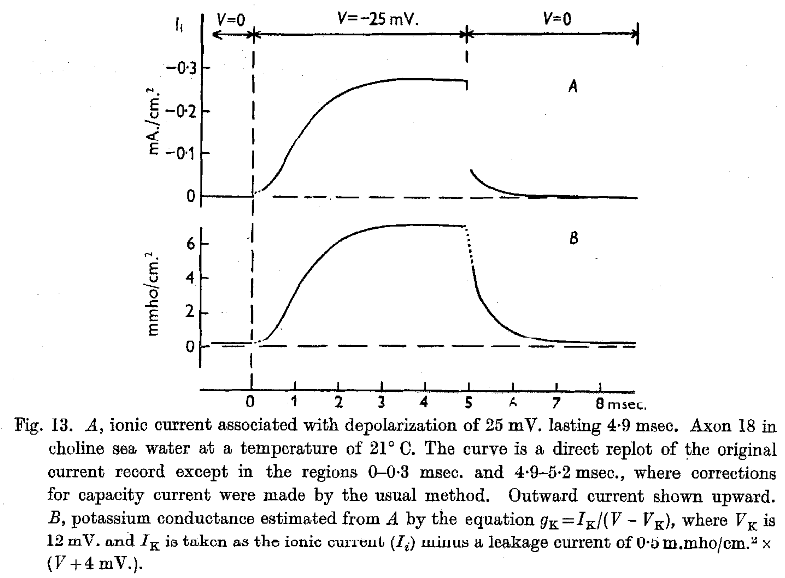
\includegraphics[width=0.8\linewidth]{potassium_current.png}
\end{figure}

\begin{itemize}
\item What functional form did Hodgkin and Huxley assume for the potassium conductance?
\item What dynamical equation governs the gating variable used in this model?
\end{itemize}

Write down these two equations. Then verify (without substituting numerical values) that this assumption indeed leads to fourth-order dynamics at the onset of the current and first-order dynamics at the end of the record.

\begin{solution}
\textbf{Assumed functional form.}
Hodgkin and Huxley modeled the macroscopic potassium conductance as
\begin{equation}
g_K(t)=\bar g_K\,n^4(t),
\end{equation}
where $\bar g_K$ is the maximal conductance and $n\in[0,1]$ is an activation (gating) variable.

\textbf{Gating dynamics.}
For a fixed membrane voltage $V$ (voltage clamp), the gating variable follows a first-order kinetic equation
\begin{equation}
\frac{\mathrm{d}n}{\mathrm{d}t}=\alpha_n(V)\,(1-n)-\beta_n(V)\,n
\;=\;\frac{n_\infty(V)-n}{\tau_n(V)},
\end{equation}
with
\begin{equation}
n_\infty(V)=\frac{\alpha_n(V)}{\alpha_n(V)+\beta_n(V)},
\qquad
\tau_n(V)=\frac{1}{\alpha_n(V)+\beta_n(V)}.
\end{equation}

\textbf{Onset: fourth-order onset from $n^4$, and the early-time first-order approximation.}
Under a depolarizing step, $n(t)=n_\infty\bigl(1-\mathrm{e}^{-t/\tau_n}\bigr)$ (assuming $n(0)=0$), hence
\begin{equation}
g_K(t)=\bar g_K\,n_\infty^4\bigl(1-\mathrm{e}^{-t/\tau_n}\bigr)^4.
\end{equation}
For very early time $t\ll \tau_n$, the underlying first-order ODE reduces to
\begin{equation}
\tau_n\,\frac{\mathrm{d}n}{\mathrm{d}t}=n_\infty-n\ \approx\ n_\infty
\quad\Longrightarrow\quad
\frac{\mathrm{d}n}{\mathrm{d}t}\approx \frac{n_\infty}{\tau_n},
\end{equation}
so $n(t)\approx (n_\infty/\tau_n)t$ and therefore
\begin{equation}
g_K(t)\approx \bar g_K\,\left(\frac{n_\infty}{\tau_n}\right)^4 t^4
\qquad (t\to 0),
\end{equation}
which explains why a fourth-order onset is needed to capture the initial delay in $g_K$.

\textbf{Tail: first-order decay, and an explicit first-order ODE for $g_K$.}
After repolarization, $n_\infty\approx 0$ and the first-order gating ODE becomes
\begin{equation}
\tau_n\,\frac{\mathrm{d}n}{\mathrm{d}t}= -n
\quad\Longrightarrow\quad
n(t)=n(t_1)\,\mathrm{e}^{-(t-t_1)/\tau_n}.
\end{equation}
Then
\begin{equation}
g_K(t)=\bar g_K\,n^4(t)=g_K(t_1)\,\mathrm{e}^{-4(t-t_1)/\tau_n},
\end{equation}
which equivalently satisfies a \emph{first-order} ODE in $g_K$ itself:
\begin{equation}
\frac{\mathrm{d}g_K}{\mathrm{d}t}=-\frac{4}{\tau_n}\,g_K.
\end{equation}
\end{solution}
\clearpage

\section{Implementation Details in Numerical Simulation of HH Model}

Before attempting this problem, please make sure you have read the Chapter 3 of the lecture notes.

\subsection{Avoiding 0/0 in Numerical Computation}

We have already introduced the empirical expressions for the transition
rates of the gating variables (assuming a resting potential
$V_{\text{rest}}=\SI{-65}{\milli\volt}$):

\[
{\renewcommand{\arraystretch}{2}
\begin{array}{l l}
\alpha_n(V) = 0.01\cdot\dfrac{V+55}{1-\mathrm{e}^{-\frac{V+55}{10}}}
&
\beta_n(V)=0.125\,\mathrm{e}^{-\frac{V+65}{80}}
\\
\alpha_m(V) = 0.1\cdot\dfrac{V+40}{1-\mathrm{e}^{-\frac{V+40}{10}}}
&
\beta_m(V) = 4\,\mathrm{e}^{-\frac{V+65}{18}}
\\
\alpha_h(V) = 0.07\,\mathrm{e}^{-\frac{V+65}{20}}
&
\beta_h(V) = \dfrac{1}{1+\mathrm{e}^{-\frac{V+35}{10}}}
\end{array}}
\]

When examining these formulas, you may wonder what happens if one directly
substitutes $V=\SI{-55}{\milli\volt}$ into the expression for $\alpha_n(V)$.
In this case, both the numerator and denominator become zero,
leading to an indeterminate form. Mathematically, the limit as
$V\to\SI{-55}{\milli\volt}$ does exist and is finite.
However, in numerical computation this expression is problematic:
when $x$ is very small, $\exp(x)$ is extremely close to 1,
and subtracting 1 leads to \emph{catastrophic cancellation}.
This may result in large numerical errors, loss of precision,
or even NaN values. 
To avoid this issue, simulators often replace the original expression
with a numerically stable approximation near the singular point.

We formalize this idea by defining

\[
\operatorname{vtrap}(x,y)=
\begin{cases}
\dfrac{x}{\mathrm{e}^{\frac{x}{y}}-1},
&\left|\dfrac{x}{y}\right|>10^{-6}
\\[6pt]
f(x,y),
&\text{otherwise.}
\end{cases}
\]

\textbf{Tasks}

\begin{enumerate}
\item Derive the expression for $f(x,y)$.

\textit{Hint:} perform a variable substitution and use a Taylor expansion.
You may use the identity
\[
\frac{1}{1+z+O(z^2)}=1-z+O(z^2).
\]

\item Among the six rate expressions above, identify those that require
the approximation near the singular point, and rewrite them using the
$\operatorname{vtrap}$ function.
\end{enumerate}

\begin{solution}
\textbf{1) Derive $f(x,y)$ (Taylor expansion near $x/y=0$).}
Start from
\[
\operatorname{vtrap}(x,y)=\frac{x}{\mathrm{e}^{x/y}-1}.
\]
Use the dimensionless substitution $z:=x/y$ (so $x=yz$). It is often helpful to view this as
\[
\operatorname{vtrap}(x,y)=y\,g(z),\qquad g(z):=\frac{z}{\mathrm{e}^{z}-1},\qquad z=\frac{x}{y},
\]
so we only need to expand the single-variable function $g(z)$ near $z=0$.
\[
\operatorname{vtrap}(x,y)=\frac{yz}{\mathrm{e}^{z}-1}\ \equiv\ \operatorname{vtrap}(y,z),
\]
Taylor expand $\mathrm{e}^{z}$ around $z=0$:
\[
\mathrm{e}^{z}-1=z+\frac{z^2}{2}+\frac{z^3}{6}+O(z^4)=z\left(1+\frac{z}{2}+\frac{z^2}{6}+O(z^3)\right).
\]
Therefore
\[
\frac{z}{\mathrm{e}^{z}-1}=\frac{1}{1+\frac{z}{2}+\frac{z^2}{6}+O(z^3)}
=1-\frac{z}{2}+\frac{z^2}{12}+O(z^3),
\]
and hence
\begin{equation}
\operatorname{vtrap}(x,y)=y\left(1-\frac{z}{2}+\frac{z^2}{12}+O(z^3)\right)
=y-\frac{x}{2}+O\!\left(\frac{x^2}{y}\right).
\end{equation}
In particular, if we keep the \emph{first-order} term in $x$ (which already requires using the \emph{second-order} Taylor expansion $\mathrm{e}^{z}=1+z+\tfrac{z^2}{2}+O(z^3)$ to control the cancellation), we obtain the approximation
\begin{equation}
f(x,y)=y-\frac{x}{2}
\qquad\bigl(|x/y|\le 10^{-6}\bigr),
\end{equation}
with truncation error on the order of $O(x^2/y)$.

\textbf{2) Which rates need $\operatorname{vtrap}$, and how to rewrite them.}
The problematic (0/0) forms occur when the numerator is zero and simultaneously the exponential term makes the denominator zero.
From the given formulas, this happens at:
\[
\alpha_n(V):\ V=\SI{-55}{\milli\volt},
\qquad
\alpha_m(V):\ V=\SI{-40}{\milli\volt}.
\]
The other four rates are nonsingular.

Using the provided definition $\operatorname{vtrap}(x,y)=\dfrac{x}{\mathrm{e}^{x/y}-1}$, we can rewrite the two rates \emph{exactly} as
\begin{equation}
\alpha_n(V)=0.01\,\frac{V+55}{1-\mathrm{e}^{-(V+55)/10}}
=0.01\,\operatorname{vtrap}(-(V+55),10),
\end{equation}
\begin{equation}
\alpha_m(V)=0.1\,\frac{V+40}{1-\mathrm{e}^{-(V+40)/10}}
=0.1\,\operatorname{vtrap}(-(V+40),10).
\end{equation}
\end{solution}

\clearpage
\subsection{Temperature Correction}

Temperature affects the transition rates between the states of
the gating variables. Specifically, all transition rates are multiplied
by the factor
\[
q_{10}=3^{\frac{T_{\text{cel}}-6.3}{10}},
\]
where $T_{\text{cel}}$ is the temperature measured in \si{\degreeCelsius}.

This temperature correction means that \SI{6.3}{\degreeCelsius}
is taken as the reference temperature, and for every
\SI{10}{\degreeCelsius} increase in temperature,
the rate constants are multiplied by a factor of 3.

\textbf{Task}

Determine which parts of the original HH computational procedure
need to be modified to include the temperature correction, then write down the corrected equations (try to modify as little of the
original expressions as possible). If a formula involves $n$, $m$,
or $h$, it is sufficient to present only one representative example.

\vspace{2em}

\nosolutionpagebreak
\begin{solution}
\textbf{Baseline temperature of the original rates.}
The classic Hodgkin--Huxley rate formulas $\alpha(V),\beta(V)$ were fitted to squid giant axon data at the reference temperature
$T_{\text{ref}}=\SI{6.3}{\degreeCelsius}$. In this handout, the uncorrected $\alpha_n,\beta_n,\alpha_m,\beta_m,\alpha_h,\beta_h$ should therefore be interpreted as rates at $\SI{6.3}{\degreeCelsius}$.

\textbf{What changes under temperature correction.}
Temperature correction scales \emph{transition rates} (units: $\mathrm{ms}^{-1}$). Thus we modify only the rate functions used in the gating-variable ODE updates:
\begin{equation}
q_{10}=3^{\frac{T_{\text{cel}}-T_{\text{ref}}}{10}}=3^{\frac{T_{\text{cel}}-6.3}{10}},
\qquad
\alpha_x^{(T)}(V)=q_{10}\,\alpha_x(V),\ \beta_x^{(T)}(V)=q_{10}\,\beta_x(V),
\end{equation}
where $x\in\{n,m,h\}$. It is sufficient to show one representative example; below we use $n$.

\textbf{Representative example (for $n$).}
The corrected gating ODE can be written as
\begin{equation}
\frac{\mathrm{d}n}{\mathrm{d}t}=\alpha_n^{(T)}(V)(1-n)-\beta_n^{(T)}(V)n
=q_{10}\bigl[\alpha_n(V)(1-n)-\beta_n(V)n\bigr].
\end{equation}
Equivalently, in $n_\infty$--$\tau_n$ form,
\begin{equation}
n_\infty^{(T)}(V)=\frac{\alpha_n^{(T)}}{\alpha_n^{(T)}+\beta_n^{(T)}}
=\frac{\alpha_n}{\alpha_n+\beta_n}=n_\infty(V),
\qquad
\tau_n^{(T)}(V)=\frac{1}{\alpha_n^{(T)}+\beta_n^{(T)}}=\frac{\tau_n(V)}{q_{10}}.
\end{equation}

\textbf{Impact on the computation.}
Compared with the uncorrected procedure, $n_\infty$ (and similarly $m_\infty,h_\infty$) is unchanged, but the time constants shrink by $q_{10}$.
This accelerates gating dynamics, which in turn makes $g_K(t)=\bar g_K n^4$ and $g_{\mathrm{Na}}(t)=\bar g_{\mathrm{Na}} m^3 h$ evolve faster; the membrane equation itself is unchanged except through these faster-evolving conductances.
\end{solution}

\clearpage

\section{From Single Channels to Macroscopic Conductance}

Real ion channels often have multiple microscopic states. 
For example, a channel may occupy several closed states ($C_1,C_2,\dots$), 
one or more open states ($O$), and inactivated states ($I_1,I_2,\dots$).
Transitions between these states occur randomly.

In a Markov description, if the channel is currently in state $i$, 
the probability of transitioning to state $j$ within a short time $dt$ is
$k_{ij}(V)\,dt$, where $k_{ij}(V)$ is a voltage-dependent rate.

Let $p_i(t)$ denote the probability that the channel is in state $i$ at time $t$.
Then

\[
\frac{dp_i}{dt} = \sum_{j\ne i} p_j k_{ji} - p_i \sum_{j\ne i} k_{ij}.
\]

Suppose the set of open states is $\mathcal O$. The open probability is

\[
P_O(t)=\sum_{i\in\mathcal O} p_i(t).
\]

Now assume the membrane contains $N$ identical channels, each with
single-channel conductance $\gamma$.

\begin{enumerate}
\item Write the total conductance $g(t)$ of this channel population in terms of $P_O(t)$,
and \textbf{briefly} explain why the macroscopic conductance can be interpreted as the
\emph{average behavior} of many stochastic single-channel openings. 

\textit{Hint:} Distinguish carefully between the probability that a single channel is open and the fraction of open channels in a large population.

\item Based on this argument, \textbf{briefly} explain how the gating variables used in the
Hodgkin–Huxley model can be understood as macroscopic quantities arising
from microscopic channel dynamics.
\end{enumerate}

\begin{solution}
\textbf{Matrix (Markov) formulation of single-channel kinetics.}
Collect the state probabilities into a column vector
\(
\mathbf p(t):=(p_1(t),\dots,p_M(t))^\top,\quad \sum_{i=1}^M p_i(t)=1.
\)
Define the voltage-dependent \emph{generator} matrix \(\mathbf Q(V)\in\mathbb R^{M\times M}\) by
\[
Q_{ij}(V)=k_{ji}(V)\ (i\neq j),\qquad
Q_{ii}(V)=-\sum_{j\neq i}k_{ij}(V),
\]
so each column sums to zero and probability is conserved. Then the master equation can be written compactly as
\begin{equation}
\frac{\mathrm d\mathbf p}{\mathrm dt}=\mathbf Q(V)\,\mathbf p.
\end{equation}
Let \(\mathcal O\) be the set of open states and define an \emph{open-state indicator} vector \(\mathbf c\in\{0,1\}^M\) with
\(c_i=1\) if \(i\in\mathcal O\) and \(c_i=0\) otherwise. Then
\begin{equation}
P_O(t)=\sum_{i\in\mathcal O}p_i(t)=\mathbf c^\top \mathbf p(t).
\end{equation}

\textbf{1) Macroscopic conductance as an average over many channels.}
For a population of \(N\) identical and (approximately) independent channels with single-channel conductance \(\gamma\), let \(X_r(t)\in\{0,1\}\) indicate whether channel \(r\) is open at time \(t\).
Then the instantaneous number of open channels is \(N_O(t)=\sum_{r=1}^N X_r(t)\), and the total conductance is
\begin{equation}
g(t)=\gamma\,N_O(t)=N\gamma\,\underbrace{\frac{1}{N}\sum_{r=1}^N X_r(t)}_{\text{fraction open}}.
\end{equation}
Because each channel has \(\Pr[X_r(t)=1]=P_O(t)\), we have
\(
\mathbb E\bigl[\tfrac{1}{N}\sum_r X_r(t)\bigr]=P_O(t)
\)
and therefore
\begin{equation}
\mathbb E[g(t)]=N\gamma\,P_O(t)=N\gamma\,\mathbf c^\top\mathbf p(t).
\end{equation}
Moreover, by the law of large numbers the empirical fraction open converges to \(P_O(t)\) as \(N\to\infty\), with fluctuations that scale like \(\mathrm{std}\sim 1/\sqrt{N}\). Hence, for large populations, the macroscopic conductance is well-approximated by the \emph{mean-field} quantity
\begin{equation}
g(t)\approx N\gamma\,P_O(t).
\end{equation}

\textbf{2) Connecting the $\mathbf Q$-matrix view to HH $\alpha,\beta$ (concise).}
The full Markov model uses a (possibly high-dimensional) generator $\mathbf Q(V)$ to evolve state probabilities via $\dot{\mathbf p}=\mathbf Q(V)\mathbf p$.
The HH approximation replaces this detailed $\mathbf Q(V)$ by one (or several) \emph{effective two-state gates} whose generator is
\[
\mathbf Q_{\text{gate}}(V)=
\begin{pmatrix}
-\alpha(V) & \beta(V)\\
\alpha(V) & -\beta(V)
\end{pmatrix},
\qquad
\frac{\mathrm d}{\mathrm dt}
\begin{pmatrix}p_C\\p_O\end{pmatrix}=\mathbf Q_{\text{gate}}(V)
\begin{pmatrix}p_C\\p_O\end{pmatrix}.
\]
Reading off the open probability $x(t):=p_O(t)$ immediately gives
\[
\dot x=\alpha(V)(1-x)-\beta(V)x,
\]
so $\alpha,\beta$ are simply the opening/closing transition rates in this reduced $\mathbf Q$.
Assuming multiple independent gates must be permissive then yields channel open probabilities like $P_O\approx n^4$ (K) and $P_O\approx m^3h$ (Na), which is exactly why HH writes $g_K=\bar g_K n^4$ and $g_{\mathrm{Na}}=\bar g_{\mathrm{Na}} m^3h$.
\end{solution}
\clearpage

\section{Qualitative Understanding of the Hodgkin--Huxley Dynamics}

An action potential is a rapid change in membrane potential produced by the interaction between membrane voltage and voltage-gated ion channels. 
In the Hodgkin--Huxley model, we focus on how the sodium and potassium gating variables evolve over time and, in turn, shape the voltage trajectory.

\begin{figure}[H]
    \centering
    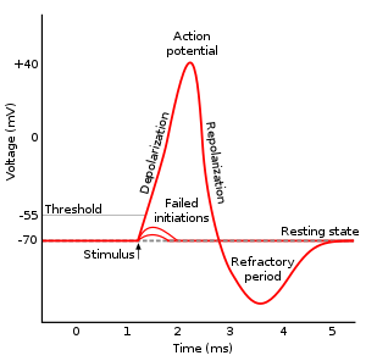
\includegraphics[width=0.3\linewidth]{AP.png}
\end{figure}

In this problem, you do \textbf{not} need to give a mathematically complete or perfectly precise explanation. 
Instead, based on your current understanding of the Hodgkin--Huxley model, \textbf{briefly} describe how the dynamics of the gating variables and the membrane potential are intertwined during a single action potential.

You may discuss, for example:
\begin{itemize}
    \item how depolarization affects the gating variables;
    \item how changes in the gating variables feed back onto the membrane potential;
    \item why the action potential rises, falls, and is followed by a refractory or afterhyperpolarized phase.
\end{itemize}

A concise qualitative explanation is sufficient. What matters most is that your answer reflects a genuine understanding of the model.

We will explore this dynamical system directly in the next lab session, so this question is intended mainly as a first attempt at building intuition.

\vspace{2em}

\nosolutionpagebreak
\begin{solution}
\textbf{Goal (what the HH model adds beyond a passive membrane).}
From the membrane equation alone, we can predict the \emph{voltage response} to a \emph{prescribed} set of currents/conductances: the voltage ``follows'' whatever ionic and applied currents we put into the equation.
However, this passive viewpoint does not yet explain why a small depolarization can turn into an all-or-none, transient impulse (an action potential) that can keep affecting downstream membrane current.

The key missing link is a mechanistic rule for how \emph{voltage changes the currents themselves}.
This is exactly the motivation of the HH model: it introduces a small number of macroscopic gating variables whose voltage-driven dynamics represent (in an averaged/statistical sense) microscopic ion-channel state transitions.
Once $V$ can drive the gates and the gates can reshape conductances, the membrane equation becomes a \emph{closed feedback system} $V\to (m,h,n)\to (g_{\mathrm{Na}},g_K)\to I_{\text{ion}}\to V$, which is the minimal structure needed to produce spike-like transients.

\tcbbreak

This whole membrane-potential transition process can be decomposed into three iterative steps.

\medskip
\textbf{Step 1: Why voltage affects gating ($V\to \alpha,\beta$) --- a minimal thermodynamic/kinetic story.}
At the microscopic level, a channel (or a channel ``gate'') occupies discrete conformations, e.g. closed $C$ and open $O$.
Opening typically moves an effective \emph{gating charge} $q_g$ across the membrane electric field.
Hence the free-energy difference between states depends on voltage:
\begin{equation}
\Delta G_{CO}(V) := G_O(V)-G_C(V) \approx \Delta G_{CO}(0) - q_g\,V.
\end{equation}
The linear term $-q_gV$ is the electrostatic work of moving charge across the membrane field: if $\mathbf E\approx -\nabla \phi$ and $V=\phi_{\text{in}}-\phi_{\text{out}}$, then $\Delta W\approx -q_g\!\int \mathbf E\cdot \mathrm d\boldsymbol\ell = -q_g V$.
Thermodynamics then gives a Boltzmann equilibrium bias
\begin{equation}
\frac{P_O^{\mathrm{eq}}(V)}{P_C^{\mathrm{eq}}(V)} = \exp\!\left(-\frac{\Delta G_{CO}(V)}{k_B T}\right),
\qquad
P_O^{\mathrm{eq}}(V)=\frac{1}{1+\exp\!\left(\frac{\Delta G_{CO}(V)}{k_B T}\right)}.
\end{equation}
To get \emph{dynamics}, we introduce opening/closing rates $\alpha(V),\beta(V)$ (units: time$^{-1}$).
At equilibrium, detailed balance for the two-state gate implies
\begin{equation}
\alpha(V)\,P_C^{\mathrm{eq}}(V)=\beta(V)\,P_O^{\mathrm{eq}}(V)
\quad\Longrightarrow\quad
\frac{\alpha(V)}{\beta(V)}=\frac{P_O^{\mathrm{eq}}(V)}{P_C^{\mathrm{eq}}(V)}
=\exp\!\left(-\frac{\Delta G_{CO}(V)}{k_B T}\right).
\end{equation}

\medskip
\textbf{Step 2: The HH ``stroke of genius'' (effective two-state, independent gates).}
HH did \emph{not} build a full multi-state Markov model from first principles; instead they introduced a compact, empirically fit, mean-field closure:
\begin{itemize}
\item Each gate is treated as an effective \emph{two-state} process with voltage-dependent rates $\alpha(V),\beta(V)$.
\item The macroscopic gating variable $x\in\{m,h,n\}$ is the open probability of that gate and obeys
\begin{equation}
\dot x=\alpha_x(V)(1-x)-\beta_x(V)x.
\end{equation}
\item Multiple gates are assumed \emph{independent} and must be permissive simultaneously, giving the conductance forms
\begin{equation}
g_{\mathrm{Na}}(V,t)=\bar g_{\mathrm{Na}}\,m^3(t)h(t),
\qquad
g_K(V,t)=\bar g_K\,n^4(t).
\end{equation}
\end{itemize}
This is the model-design leap: replace high-dimensional channel-state kinetics by a small set of voltage-driven probabilities whose products approximate the open fraction.

\medskip
\textbf{Step 3: Membrane equation as the backbone (the feedback loop that makes a spike).}
The membrane equation is the \emph{core bookkeeping law} that converts conductances into voltage dynamics:
\begin{equation}
C\,\frac{\mathrm dV}{\mathrm dt}
= I_{\mathrm{ext}}
- \bar g_{\mathrm{Na}} m^3 h\,(V-E_{\mathrm{Na}})
- \bar g_K n^4\,(V-E_K)
- g_L (V-E_L).
\end{equation}
Together with the gating ODEs, this forms a closed dynamical system. A qualitative action potential can then be read as three feedback phases:
\begin{enumerate}
\item \textbf{Upstroke (positive feedback):} a small depolarization increases $m$ (fast activation) $\Rightarrow g_{\mathrm{Na}}\uparrow$.
Because typically $V<E_{\mathrm{Na}}$, the sodium current drives further depolarization, which further increases $m$.
\item \textbf{Repolarization (negative feedback):} on a slower timescale, $h$ decreases (inactivation) and $n$ increases (K activation).
This reduces inward Na and increases outward K, pulling $V$ back down toward $E_K$.
\item \textbf{Refractory/afterhyperpolarization:} $h$ remains partially inactivated and $n$ remains elevated briefly, so the membrane is less excitable and may undershoot (toward $E_K$) until $n$ relaxes and $h$ recovers.
\end{enumerate}
In short: the membrane equation provides the voltage ``follow-the-currents'' rule, while HH supplies the missing causal link $V\to$ (gates) $\to$ (conductances) $\to$ (currents), enabling spike-like transients.
\end{solution}



\end{document}